\documentclass{beamer}
\usepackage[T1]{fontenc}
\usepackage[utf8]{inputenc}
\usepackage{hyperref}
\usepackage{graphicx}
\usepackage{caption}
\usepackage{listings}
\usepackage{color}
\usepackage{verbatim}
\usepackage{tikz}

\usetheme{Madrid}
%\usecolortheme{seahorse}
%\usecolortheme{spruce}


\AtBeginSection[]
{
    \begin{frame}
        \author{}
        \subtitle{}
        \title{\insertsection}
        \date{}
        \maketitle
        
    \end{frame}
      
    \begin{frame}
        % \frametitle{\insertsection}
        % \tableofcontents[currentsection]

        % Make a table of contents with only the current section showing the next subsections
        \frametitle{\insertsection}
        \tableofcontents[currentsection, hideothersubsections]

    \end{frame}
}


% Define the textttcolor --> blue marine
\definecolor{textttcolor}{RGB}{0, 102, 204}

% Set the default color for \texttt{}
\let\oldtexttt\texttt
\renewcommand{\texttt}[1]{\textcolor{textttcolor}{\oldtexttt{#1}}}


\title[Cloud Computing final project]{\Huge{Cloud Computing final project}}
\subtitle{A cloud-based file storage system \\ and the OSU benchmarks in k8s}
\author{Isac Pasianotto}
\date{2023-02-12}



\begin{document}

\begin{frame}
    \titlepage
\end{frame}

%%%%%%%%%%%%%%%%%%%
%%   Exercise 01 %%
%%%%%%%%%%%%%%%%%%%

\section{Cloud \textbf{basic} module}
\subsection{Requirements}

\begin{frame}
    \frametitle{Requirements}
    Identify, deploy and implement a cloud-based file storage system
    \begin{itemize}
        \item User / admin roles
        \item User should be able to login, upload, download, delete files, have a personal folder
        \item Admin should be able to manage users, quotas, etc
        \item Security evaluation
        \item Scalability evaluation
        \item Test the system with a load test
    \end{itemize}
    \begin{center}
        \begin{tabular}{cc}
            \includegraphics[height=0.2\textheight]{images/other/nextcloud-logo-extended} & \includegraphics[height=0.2\textheight]{images/other/minIO-logo}
        \end{tabular}
    \end{center}
\end{frame}


\subsection{Nextcloud: the chosen solution}
\begin{frame}
    \frametitle{Nextcloud: the chosen solution \qquad \includegraphics[height=0.09\textheight]{images/other/nextcloud-logo}}    
    \begin{itemize}
        \item Comes with already built-in all the required features (User/admin, download/upload, private folder, etc)
        \item Has a large community and a lot of plugins
        \item Can be easily deployed using docker (already available image)
        \item Supports different types of storage (local, NFS, S3, etc)
        \item Supports various database backends (MySQL, PostgreSQL, SQLite)
    \end{itemize}
\end{frame}

\begin{frame}
    \frametitle{Nextcloud: the chosen solution (con'd)}
    \begin{columns}
        \column{0.66\textwidth}
            \begin{itemize}
                \item Possibility to enable \textbf{server-side encryption}\footnote{Drawback: more CPU usage}
                \item Customizable \textbf{password minimum requirements} and \textbf{password policy}
                \item \textbf{Brute-force protection} (additional app)
                \item \textbf{Two-factor authentication}
                \item Accepts \textbf{OAuth2} external authentication
            \end{itemize}
            \textit{And what about the connection user-server?} \newline
            $\Rightarrow$ \textbf{Caddy} automatically provides a \textbf{Let's Encrypt} certificate
        \column{0.33\textwidth}
            \begin{center}
                \vspace{-4em}
                \includegraphics[height=0.45\textheight]{images/other/nextcloud-security}
                \vspace{-3em}
                \includegraphics[height=0.45\textheight]{images/other/certificate}
            \end{center}
    \end{columns}
\end{frame}

\subsection{Deployed structure}
\begin{frame}
    \frametitle{Deployed structure}
    \begin{figure}
        \includegraphics[width=\textwidth]{images/other/exbasediagram}
    \end{figure}
\end{frame}

\subsection{Load test: Locust}
\begin{frame}
    \frametitle{Load test: Locust}
    \begin{columns}
        \column{0.66\textwidth}
        \textbf{Locust} is an open-source load testing tool, which allows defining user behavior with Python code.
        \begin{itemize}
            \item start with 1 user
            \item add 1 user every second until a predefined quota is reached
            \item every second, each active user tries to perform a random task
            \item each user has a wait time between 0.5 and 3 seconds before declaring the task as failed
        \end{itemize}
        \column{0.33\textwidth}
        \begin{figure}
            \includegraphics[width=\textwidth]{images/other/locust-logo}
        \end{figure}
        \centering
        \begin{tabular}{lr}
            \hline
            Tasks & \% \\
            \hline
            upload\_small & 30\% \\
            upload\_medium & 35\% \\
            upload\_large & 5\% \\
            download & 30\%  \\
            \hline
        \end{tabular}
    \end{columns}
\end{frame}


\begin{frame}
    \frametitle{Load test: Locust (con'd)}
    
    \begin{columns}
        \column{0.66\textwidth}
        \vspace{-0.5em}
        \includegraphics[height=0.85\textheight]{images/ex1/30-users}
        \column{0.33\textwidth}
        Load test performed with server-side encryption disabled. \newline
        During the test, I got warnings from the server about the CPU usage over 90\%. \newline
        With encryption enabled, my laptop was not able to handle more tha 10 users.
    \end{columns}
 
\end{frame}

\subsection{Scalability}
\begin{frame}
    \frametitle{Scalability}
    I've considered all the possible solutions in the case of a real-world scenario
    \begin{itemize}
        \item \textbf{On-site} solution: Build on a owned server, with appropriate hardware
        \item \textbf{Infrastructure as a Service} (IaaS): rent needed resources from a cloud provider, but manage everything by yourself
        \item \textbf{Platform as a Service} (PaaS): rent a pre-configured environment, and focus only on the application and data
        \item \textbf{Software as a Service} (SaaS): rent a ready-to-use application, just use it with your data
    \end{itemize}
\end{frame}

\begin{frame}
    \frametitle{Scalability (con'd)}
    \begin{center}
        \tiny
        \begin{tabular}{l|c c c c}
                                        & \textit{on-site} & \textit{IaaS} & \textit{PaaS} & \textit{SaaS} \\
            \hline
            hardware acquisition/ cost  & high              & null      & null          & null                  \\
            maintenance costs           & high              & low       & null          & null                  \\
            predictable costs           & high              & medium    & low           & low                   \\ 
            Renting costs               & null              & low       & medium        & high                  \\
            Need to care about security & high              & medium    & on your app   & trust the vendor      \\
            Physically own the data     & yes               & no        & no            & no                    \\
            Scalability                 & completely on you & rent more resources & pay more & pay more         \\
            Time to get ready           & high              & medium    & low           & almost null           \\
        \end{tabular}
    \end{center}
\end{frame}


%%%%%%%%%%%%%%%%%%%
%%   Exercise 02 %%
%%%%%%%%%%%%%%%%%%%

\section{Cloud \textbf{advanced} module: Nextcloud in a kubernetes flavor}

\subsection{Different architecture}
\begin{frame}
    \frametitle{Different architecture}
    What is different, ...
\end{frame}

\begin{frame}
    \frametitle{Different architecture (con'd)}
    \begin{figure}
        \includegraphics[height=0.85\textheight]{images/other/exadvanceddiagram}
        %\caption{Description of the deployed structure}
    \end{figure}
\end{frame}

\subsection{How to deploy}
\begin{frame}
    \frametitle{How to deploy}
    The magic of helm
\end{frame}

\subsection{Benefits of kubernetes}
\begin{frame}
    \frametitle{Benefits of kubernetes}
    What are the benefits, ...
\end{frame}


%%%%%%%%%%%%%%%%%%%
%%   Exercise 03 %%
%%%%%%%%%%%%%%%%%%%

\section{Cloud \textbf{advanced} module: OSU benchmarks in k8s}

\subsection{Requirements}
\begin{frame}
    \frametitle{Requirements}
    \begin{itemize}
        \item 2 nodes \texttt{k8s} cluster
        \item Nodes must talk with either \texttt{Calico} or \texttt{Flannel}
        \item \texttt{MPI} operator
        \item Perform the \texttt{OSU} benchmark to evaluate the latency between the nodes
    \end{itemize}
\end{frame}

\subsection{Building the image}
\begin{frame}
    \frametitle{Building the image}
    \begin{center}
        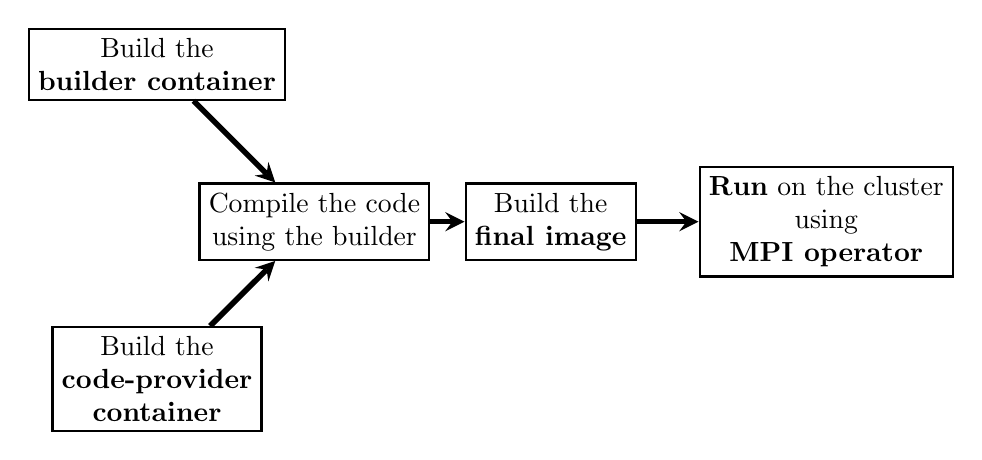
\begin{tikzpicture}
            \node[draw, thick, shape=rectangle, align=center] (A) at (0,0) {Build the  \\ \textbf{builder container}};
            \node[draw, thick, shape=rectangle, align=center] (B) at (0,-4) {Build the \\ \textbf{code-provider} \\ \textbf{container}};
            \node[draw, thick, shape=rectangle, align=center] (C) at (2,-2) {Compile the code \\ using the builder};
            \node[draw, thick, shape=rectangle, align=center] (D) at (5,-2) {Build the \\ \textbf{final image}};
            \node[draw, thick, shape=rectangle, align=center] (E) at (8.5,-2) {\textbf{Run} on the cluster \\ using \\ \textbf{MPI operator}};
            \draw[-stealth, line width=2pt] (A) -- (C);
            \draw[-stealth, line width=2pt] (B) -- (C);
            \draw[-stealth, line width=2pt] (C) -- (D);
            \draw[-stealth, line width=2pt] (D) -- (E);
        \end{tikzpicture}
    \end{center}
    \begin{tabular}{cc}
        No need to reinvent the wheel: & \includegraphics[width=0.5\textwidth]{images/other/mpidockerimage.png}
    \end{tabular}
\end{frame}

\subsection{Calico vs Flannel}
\begin{frame}
    \frametitle{Calico vs Flannel}
    From pod 0 (node 0) to pod 1 (node 1): \newline \ 

    \begin{columns}
        \column{0.5\textwidth}
        \vspace{-1.5em}
        \includegraphics[width=0.50\textwidth]{images/other/calico-logo}\newline
        \begin{figure}
            \includegraphics[width=\textwidth, height=0.5\textheight]{images/other/calico_diagram}
        \end{figure}
        \column{0.5\textwidth}
        \vspace{-1.5em}
        \includegraphics[width=0.35\textwidth]{images/other/flannel-logo}\newline
        \begin{figure}
            \includegraphics[width=\textwidth]{images/other/flannel_diagram}
        \end{figure}
    \end{columns}
\end{frame}

\subsection{results}
\begin{frame}
    \frametitle{Results\footnote{Each point represents the average of 20 runs.}}
    \begin{figure}
        \includegraphics[width=\textwidth]{images/other/calico_flannel_plot}
    \end{figure}
\end{frame}

\begin{frame}
    \frametitle{Results (con'd)}
    \begin{figure}
        \includegraphics[width=\textwidth]{images/other/one_two_node}
    \end{figure}
\end{frame}


\begin{frame}
    \frametitle{Results (con'd)}
    \begin{figure}
        \includegraphics[width=\textwidth]{images/other/calico_vs_flannel_plot}
    \end{figure}
\end{frame}



\begin{frame}
    \frametitle{\ }
    \begin{center}
        \Huge{\textbf{\textit{Thank you for your attention}}}
    \end{center}
\end{frame}

\end{document}